\documentclass{beamer}
\setbeamercovered{transparent}
\usepackage{epstopdf}
\usepackage{listings}
\usepackage{lipsum}
\usepackage{subfig}
\usepackage{algorithm}
\usepackage{algorithmicx}
\usepackage{cite}
\usepackage{lipsum}
\usepackage{amssymb}
\usepackage{color}
\usepackage{IEEEtrantools}
\usepackage{booktabs}
\usepackage{texpower}
\usepackage{amsmath}
\usepackage{caption}
\usepackage{multirow}
\usepackage{graphicx}
\newtheorem{Key points}{Key points}
\newtheorem{Summary}{Summary}
\usepackage{dblfloatfix}
%\usepackage{animate}
%\usepackage{movie15}
%\usepackage{subfig}
%\newtheorem{Definition}{Definition}
%\usepackage[font={small}]{caption}
\usepackage{beamerthemeshadow}
\newcommand\Fontvi{\fontsize{5}{6.2}\selectfont}
\newcommand\Fontvia{\fontsize{6}{7.2}\selectfont}
\newcommand\Fontviaa{\fontsize{8}{7.2}\selectfont}
%\captionsetup{font=scriptsize,labelfont=scriptsize}
 \usetheme{Antibes}%PaloAlto
\begin{document}
\title[Lecture 1]{Data Structures and Object Oriented Programming using C++} 
\author[]{Ahsan Ijaz}
\date{September 9, 2013}
 \frame{\titlepage}
% \AtBeginSection[]
% {
% \begin{frame}<beamer>{Table of Contents}
% \tableofcontents[currentsection,currentsubsection, 
%     hideothersubsections, 
%     sectionstyle=show/shaded,
% ]
% \end{frame}
% }

\section{Course Details}
\frame{\frametitle{Pre-requisite}
\textbf{Algorithm and Computing}
\begin{itemize}
\item Basic familiarity with C/C++ language
\item Data types, Variables, Arrays
\item Arithmetic/logical operastors 
\item Loops
\item Functions
\item Pointers
\item Structures
\end{itemize}
}
 %\subfloat[]{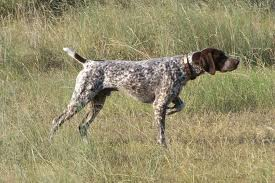
\includegraphics[width=0.3\columnwidth]{pointer.jpg}} \\
 %\subfloat[]{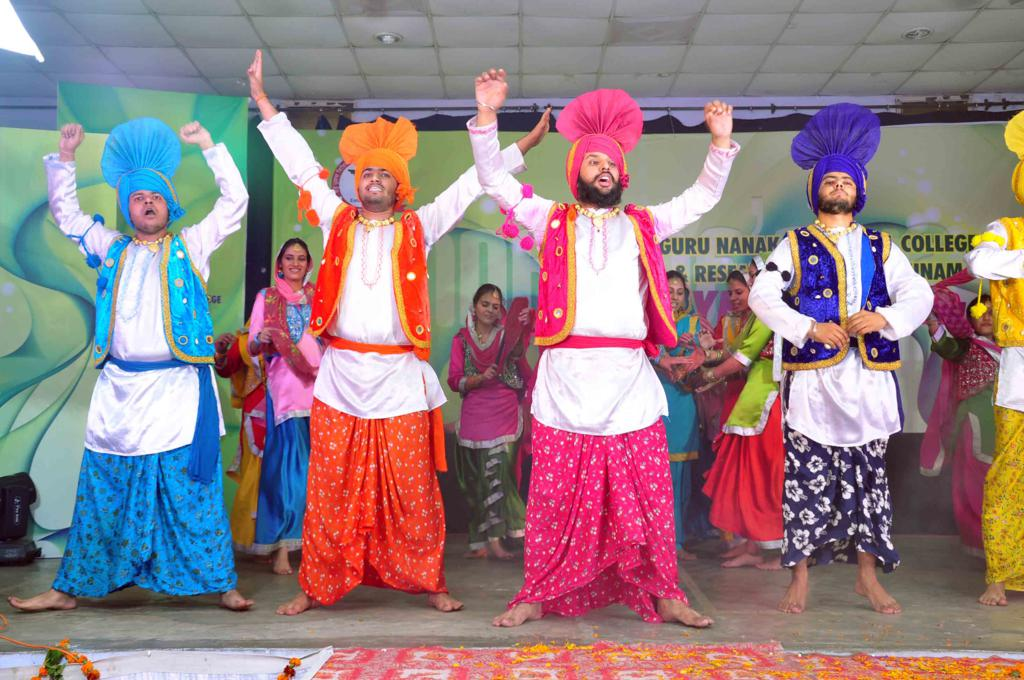
\includegraphics[width=0.3\columnwidth]{func.jpg}}
 %\subfloat[]{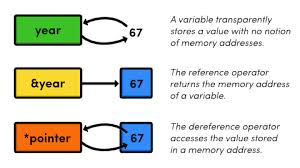
\includegraphics[width=0.3\columnwidth]{cpointer.jpg}} \\
 %\subfloat[]{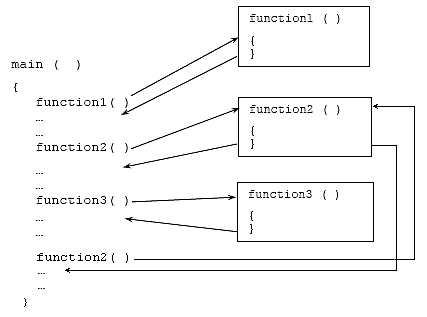
\includegraphics[width=0.3\columnwidth]{cfunc.png}}
\subsection{Quiz 0}
 \frame{\frametitle{Words to think about}
   \begin{enumerate}
   \item Loops
\item Functions
\item Pointers
\item Structure
\item Function Overloading
\item Files
   \end{enumerate}
}

\subsection{Quiz 0 Discussion}
 \frame{\frametitle{Pointers and Functions}
\begin{figure}
  \begin{tabular}{c|c}
\subfloat{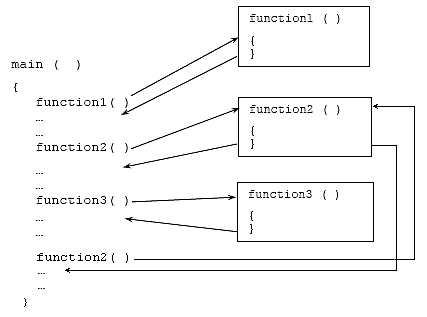
\includegraphics[width=0.3\columnwidth]{cfunc}} &
\subfloat{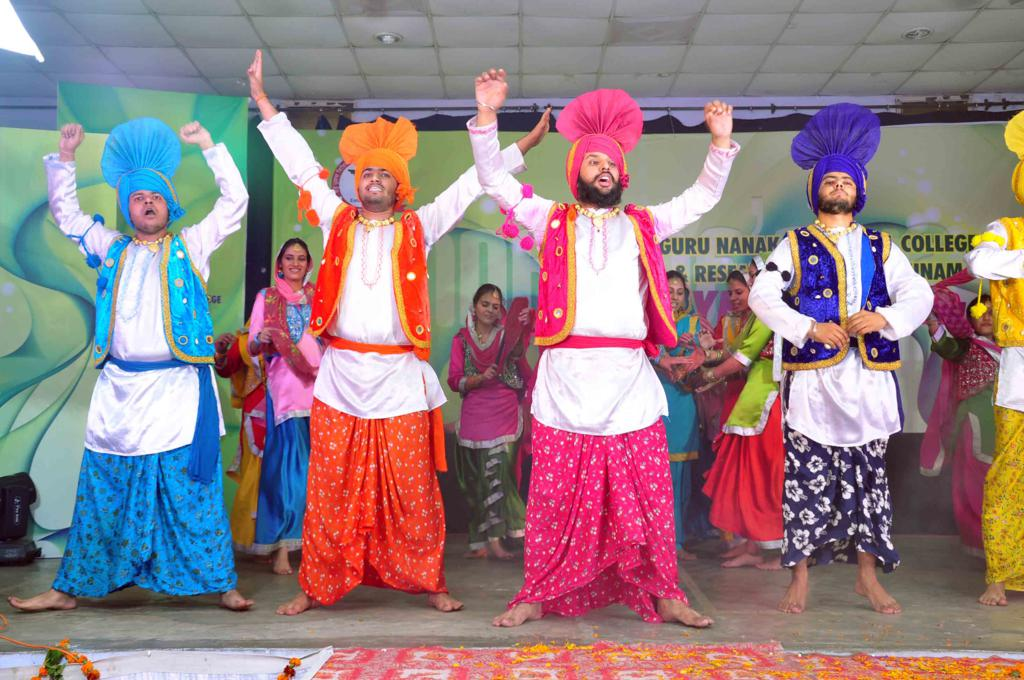
\includegraphics[width=0.3\columnwidth]{func}}
  \end{tabular}
\caption{Functions}
\end{figure}

\begin{figure}
  \begin{tabular}{c|c}
\subfloat{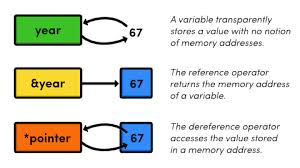
\includegraphics[width=0.3\columnwidth]{cpointer}} &
\subfloat{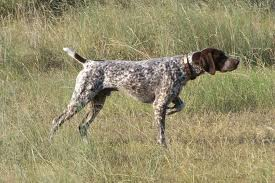
\includegraphics[width=0.25\columnwidth]{pointer}}
  \end{tabular}
\caption{Pointers}
\end{figure}
}

 \frame{\frametitle{Loops and Structures}
\begin{figure}
  \begin{tabular}{c|c}
\subfloat{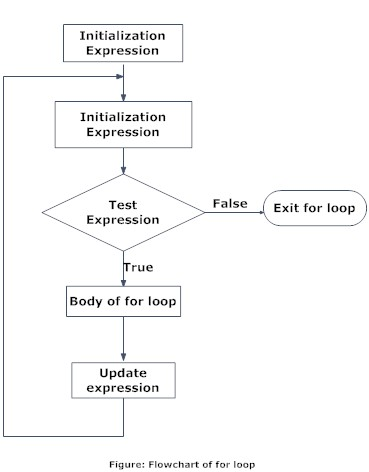
\includegraphics[width=0.1\columnwidth]{cloops}} &
\subfloat{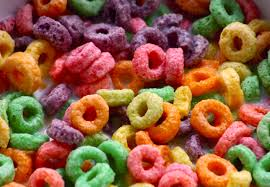
\includegraphics[width=0.3\columnwidth]{loops}}
  \end{tabular}
\caption{Loops}
\end{figure}

\begin{figure}
  \begin{tabular}{c|c}
\subfloat{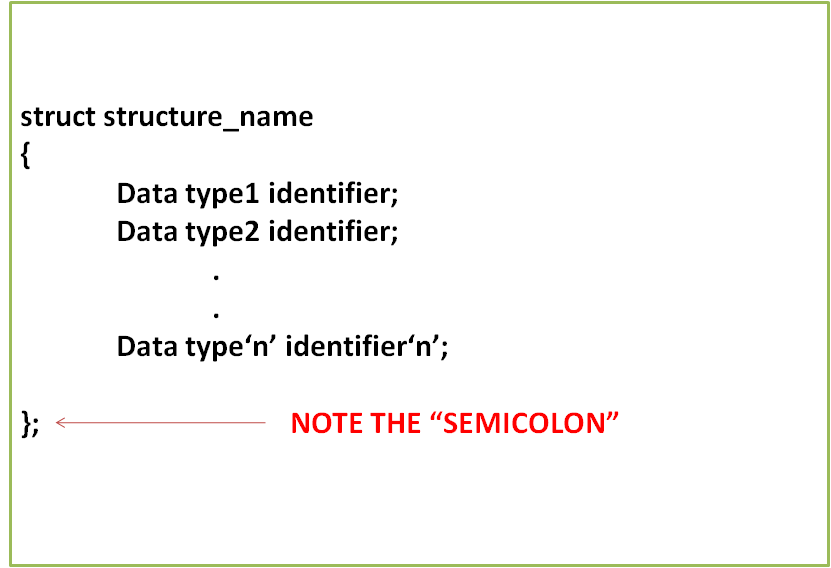
\includegraphics[width=0.23\columnwidth]{cstructure}} &
\subfloat{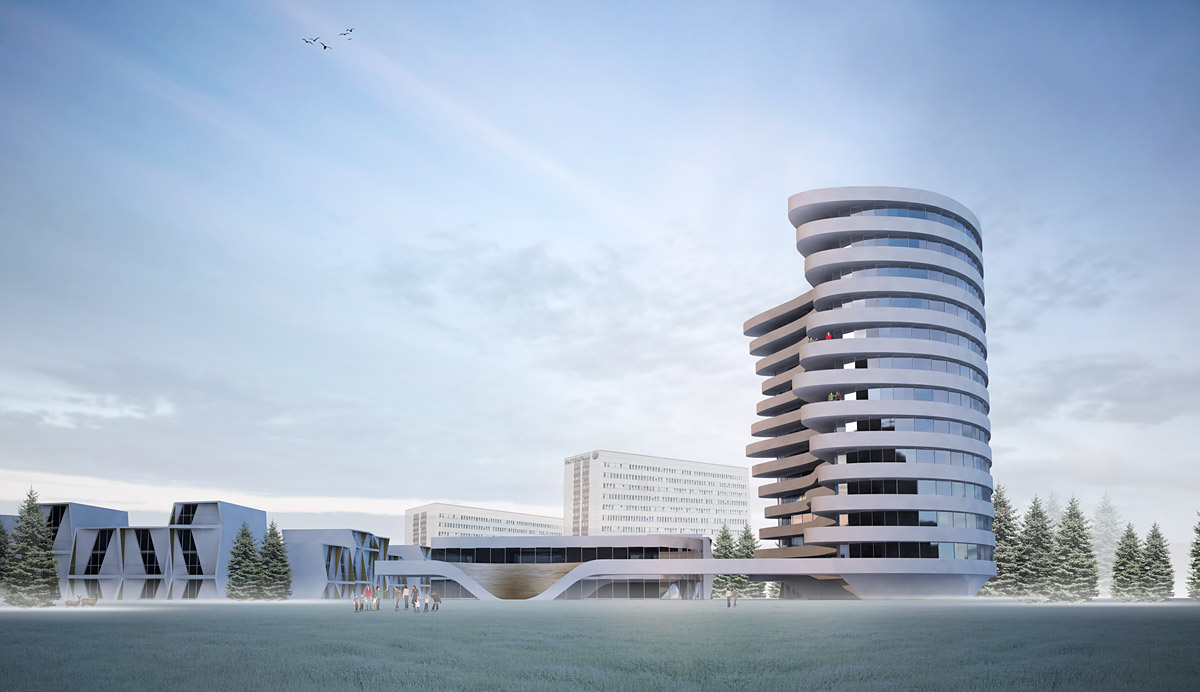
\includegraphics[width=0.27\columnwidth]{structure1}}
  \end{tabular}
\caption{Structures}
\end{figure}

}

\frame{\frametitle{Files}
\begin{figure}
\centering
\subfloat{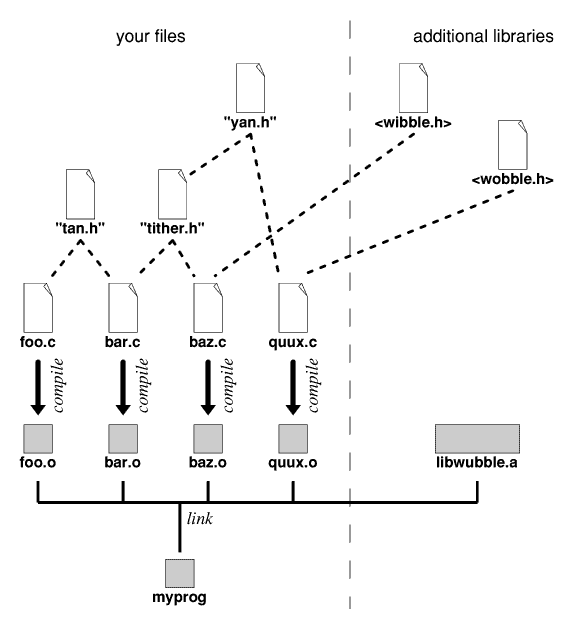
\includegraphics[width=0.4\columnwidth]{cfile}} 
\subfloat{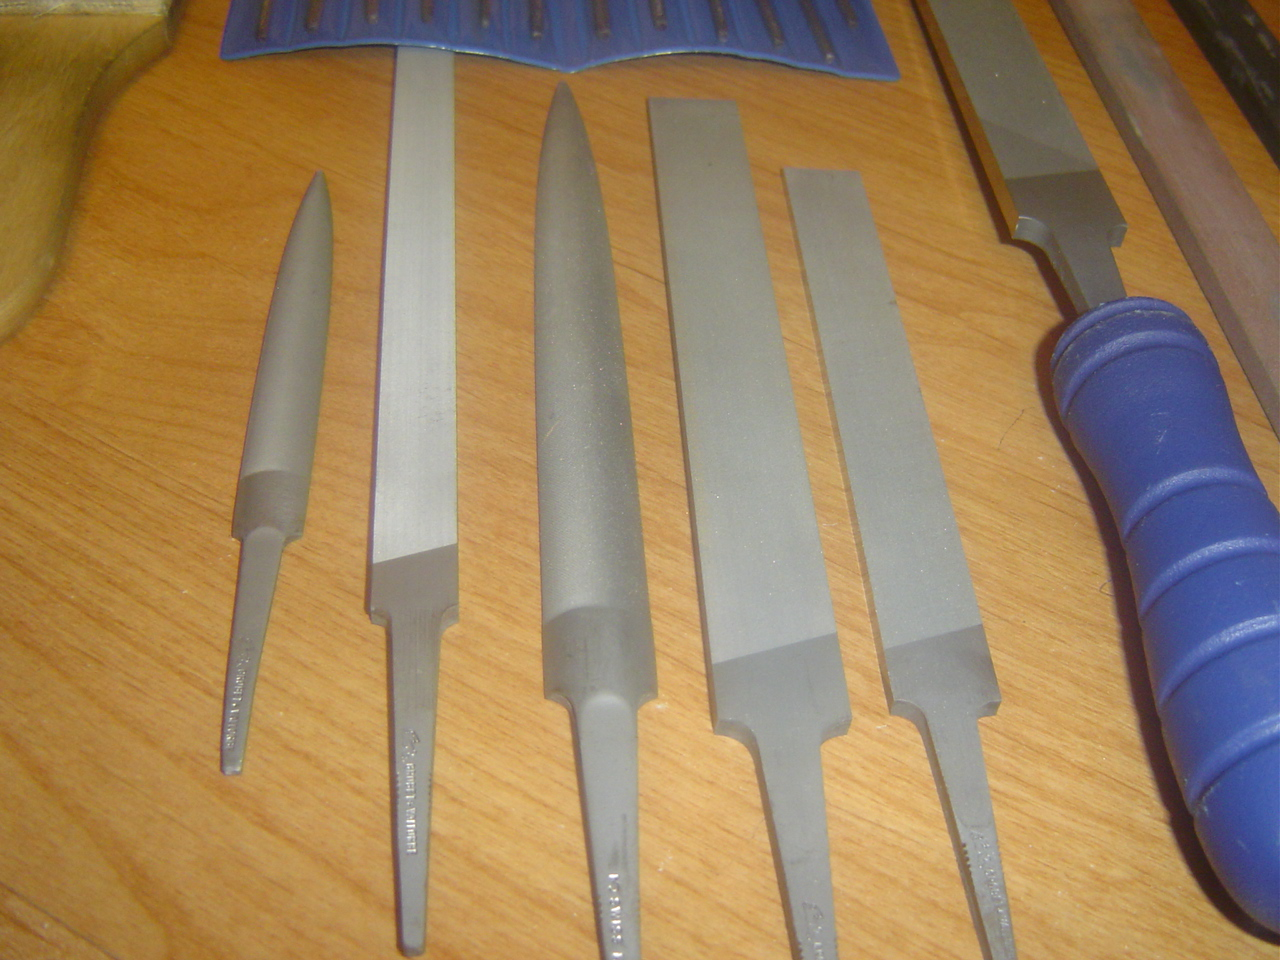
\includegraphics[width=0.5\columnwidth]{file}}
\caption{Filing}
\end{figure}
}

\frame{\frametitle{Function Overloading}
\begin{figure}
\centering
\subfloat{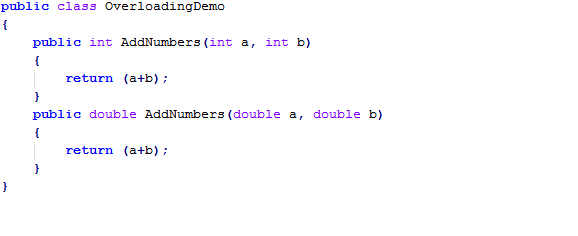
\includegraphics[width=0.7\columnwidth]{cfuno}} 
\subfloat{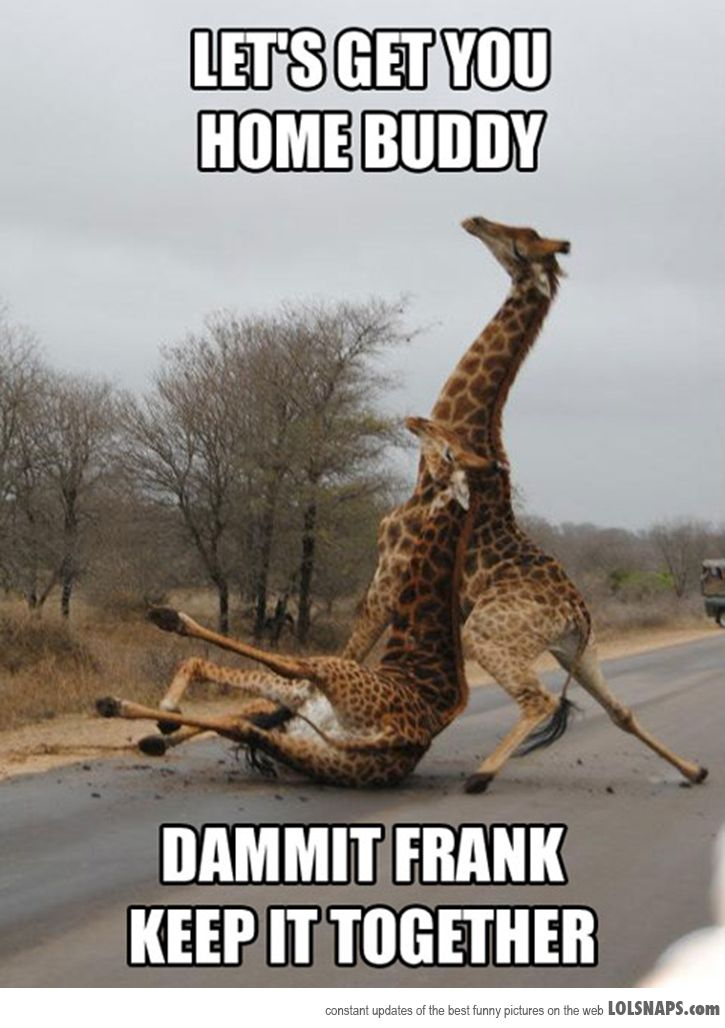
\includegraphics[width=0.3\columnwidth]{funo}}
\caption{Function Overloading}
\end{figure}
}

\frame{\frametitle{Suggested Reference Material}
  \begin{itemize}
  \item Object Oriented Programming in C++, Robert Lafore
  \item C++ How to Program, Deitel and Deitel
  \item Electronic resources will be provided
  \end{itemize}
}
\subsection{}
\frame{\frametitle{Course Objective}
  \begin{itemize}
  \item Concepts of Object oriented programming
  \item Concepts of Data Structures 
  \item Proficiency in implementing these concepts using C++
  \end{itemize}
}

\frame{\frametitle{Major topics of Course}
\textbf{Object Oriented Programming}
  \begin{itemize}
  \item Objects and Classes
  \item Self-Referential Structures
  \item Inheritance
  \item Polymorphism
\end{itemize}
\textbf{Data Structures}
  \begin{itemize}
  \item Linked Lists
  \item Stacks and Queues
  \item Trees
  \item Sorting Algorithms
  \end{itemize}
\textbf{General Topics}
  \begin{itemize}
    \item Templates
  \item Exception Handling
  \end{itemize}
}
\frame{\frametitle{Grading (consider tentative)}
\textbf{Class Distribution}
  \begin{itemize}
  \item Finals 40\%
  \item Mid terms 25\%
   \item Quizes 15\%
  \item Projects 20\%
  \end{itemize}
}
\section{Thinking Objects}
\frame{\frametitle{Languages}
  \begin{definition}
The method of human communication, either spoken or written, consisting of the use of words in a structured and conventional way.    
  \end{definition}
\textbf{Programming Languages}
\begin{enumerate}
\item Java
\item Python
\item C and C++
\item FORTRAN
\item Elisp
\item PHP
\item Many more
\end{enumerate}
}
\subsection{Class Exercise 1}
\frame{\frametitle{'Objectify' your Friend}
A natural way of thinking. Think about representing any of your friend:
\textbf{Example parameters:}
\begin{itemize}
\item Name
\item Age 
\item Height
\item Shared Experience
\item One word Description
\item Emotional state
\item Social Profile
\item Convincing/reading/writing/speaking skills
\item Eye color, hair, cloth $\cdots$
\item Sports
\item Habits
\item Abilities
\end{itemize}
(Data type: int, string, float?? )\\


}
\subsection{}
\frame{\frametitle{Objects}
% \begin{columns}[onlytextwidth]
%     \begin{column}{0.6\textwidth}
%       \centering
Defining Problems using Objects.
  \begin{itemize}
  \item Characteristics
  \item Responsibilities
  \end{itemize}
\begin{figure}
%includegraphics[width=2\columnwidth]{aaaorig.png}\\
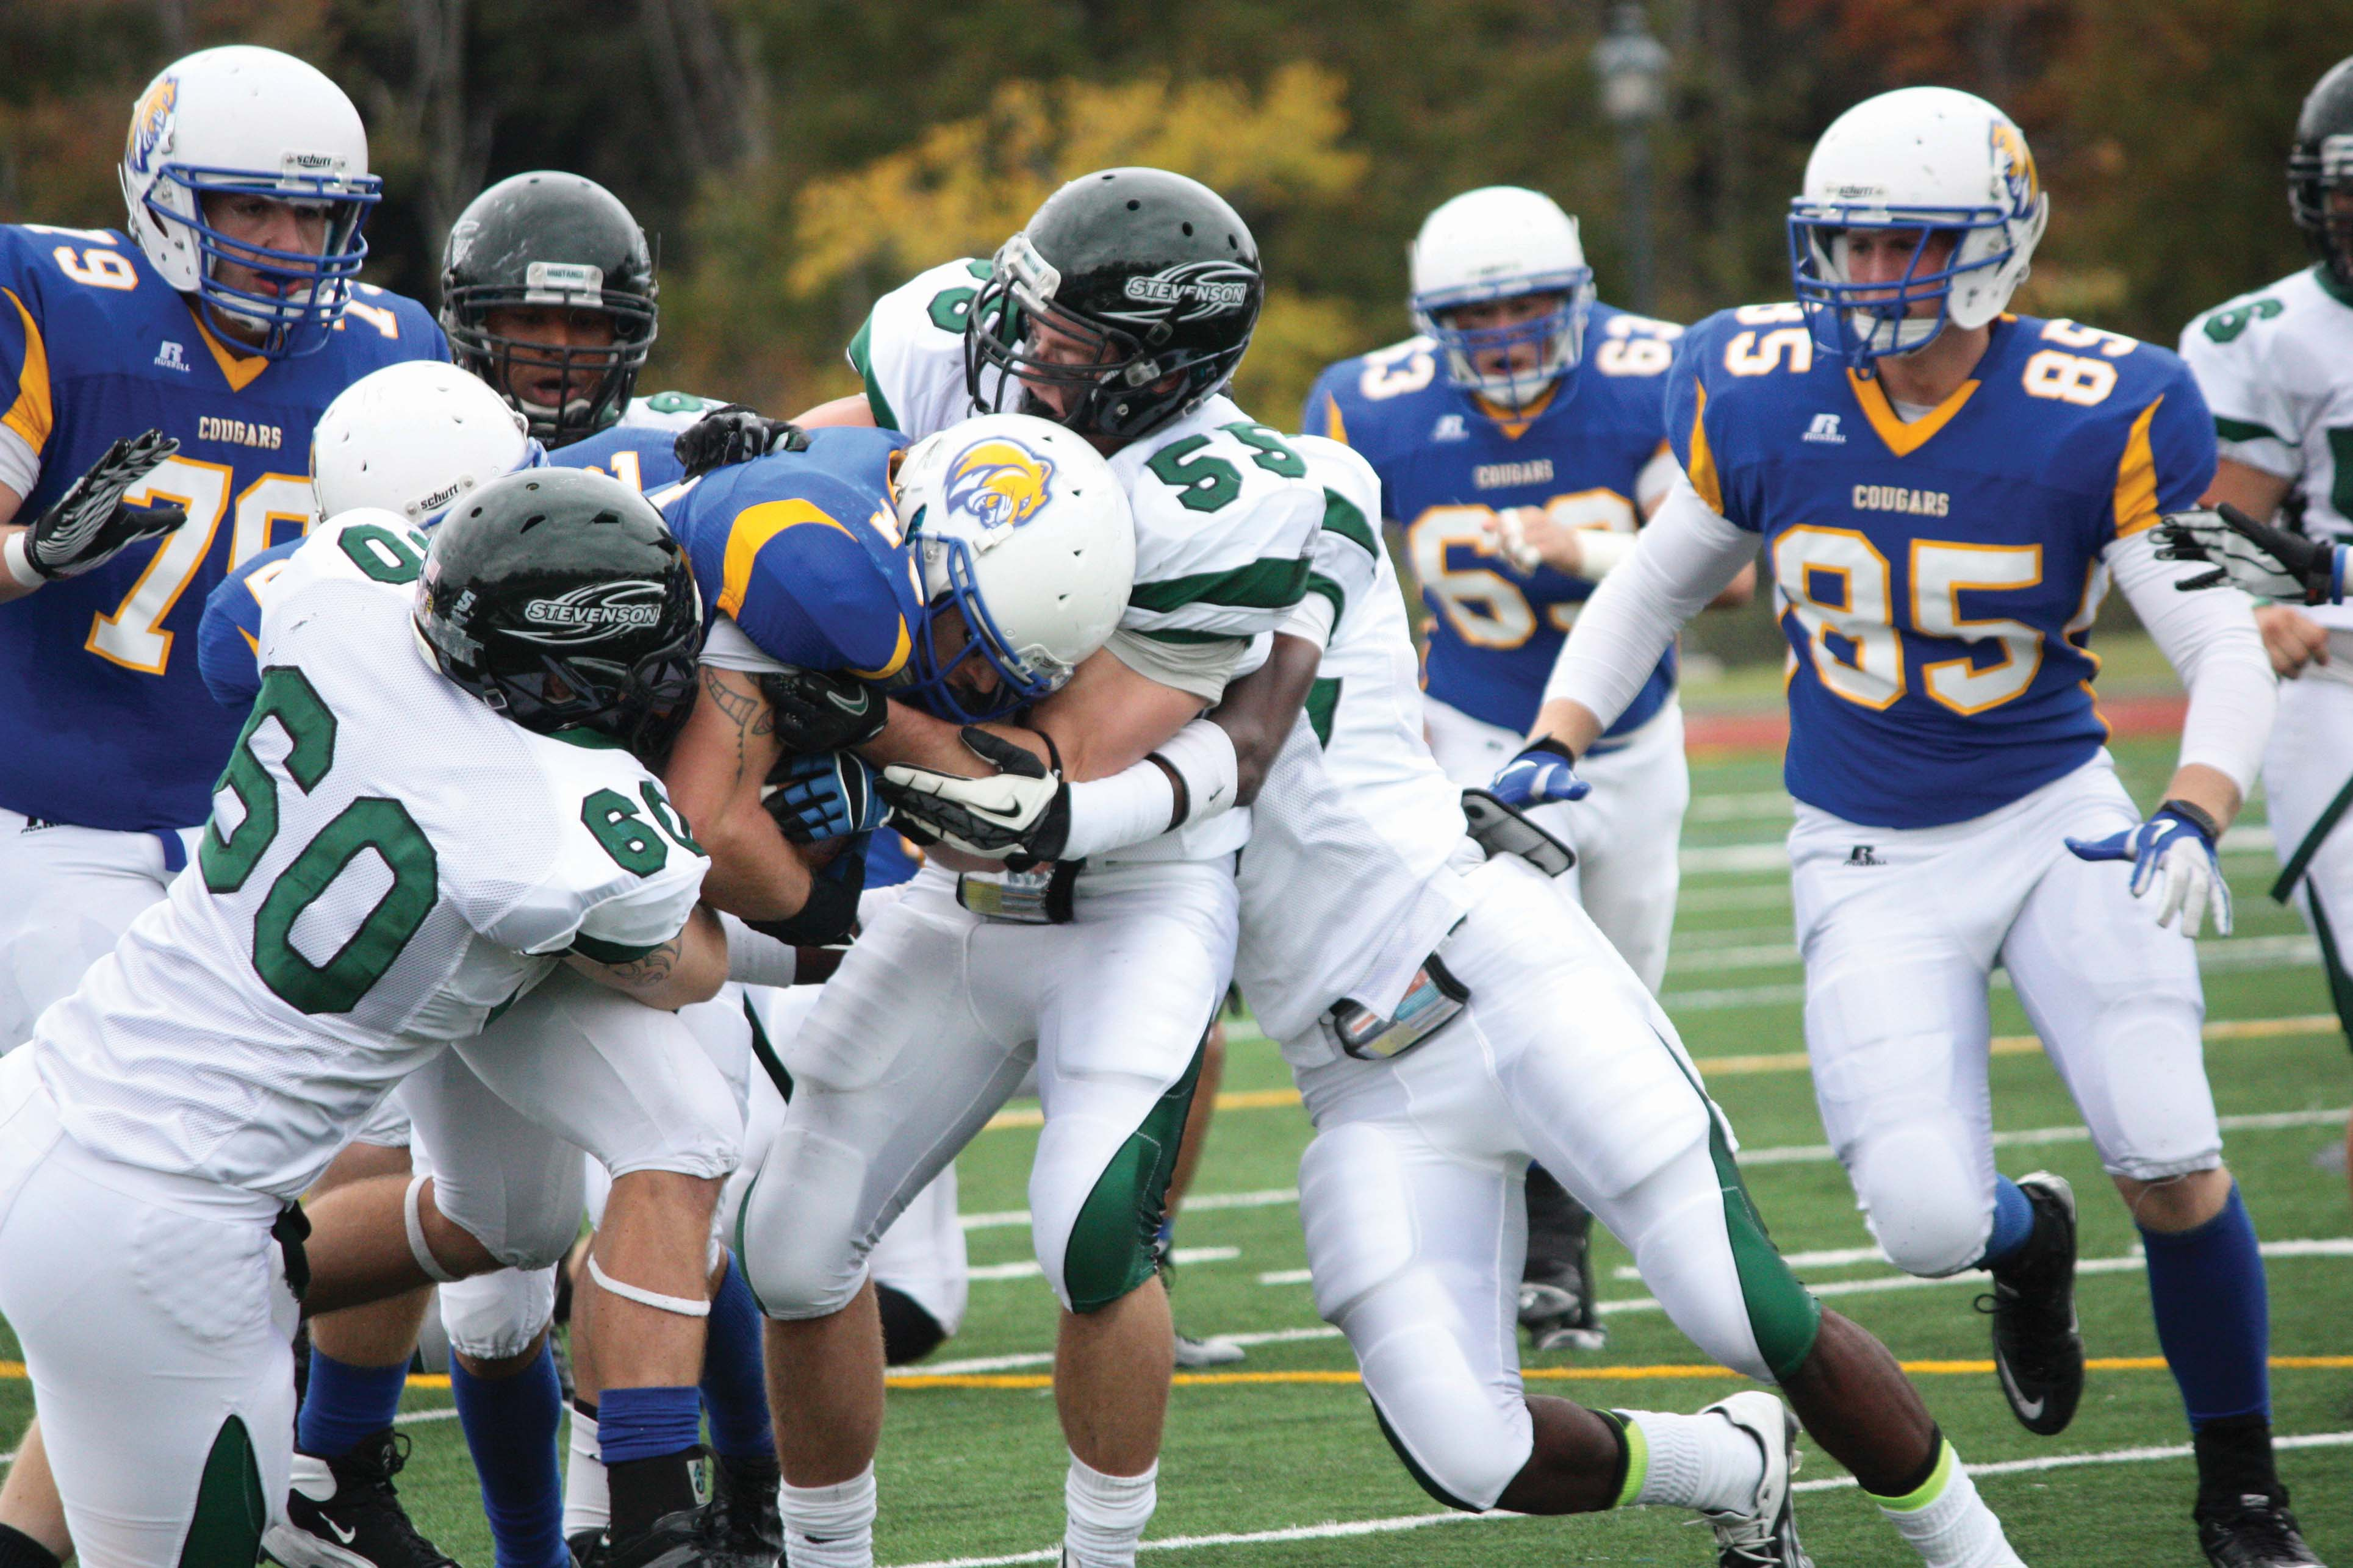
\includegraphics[width=0.3\columnwidth]{football}
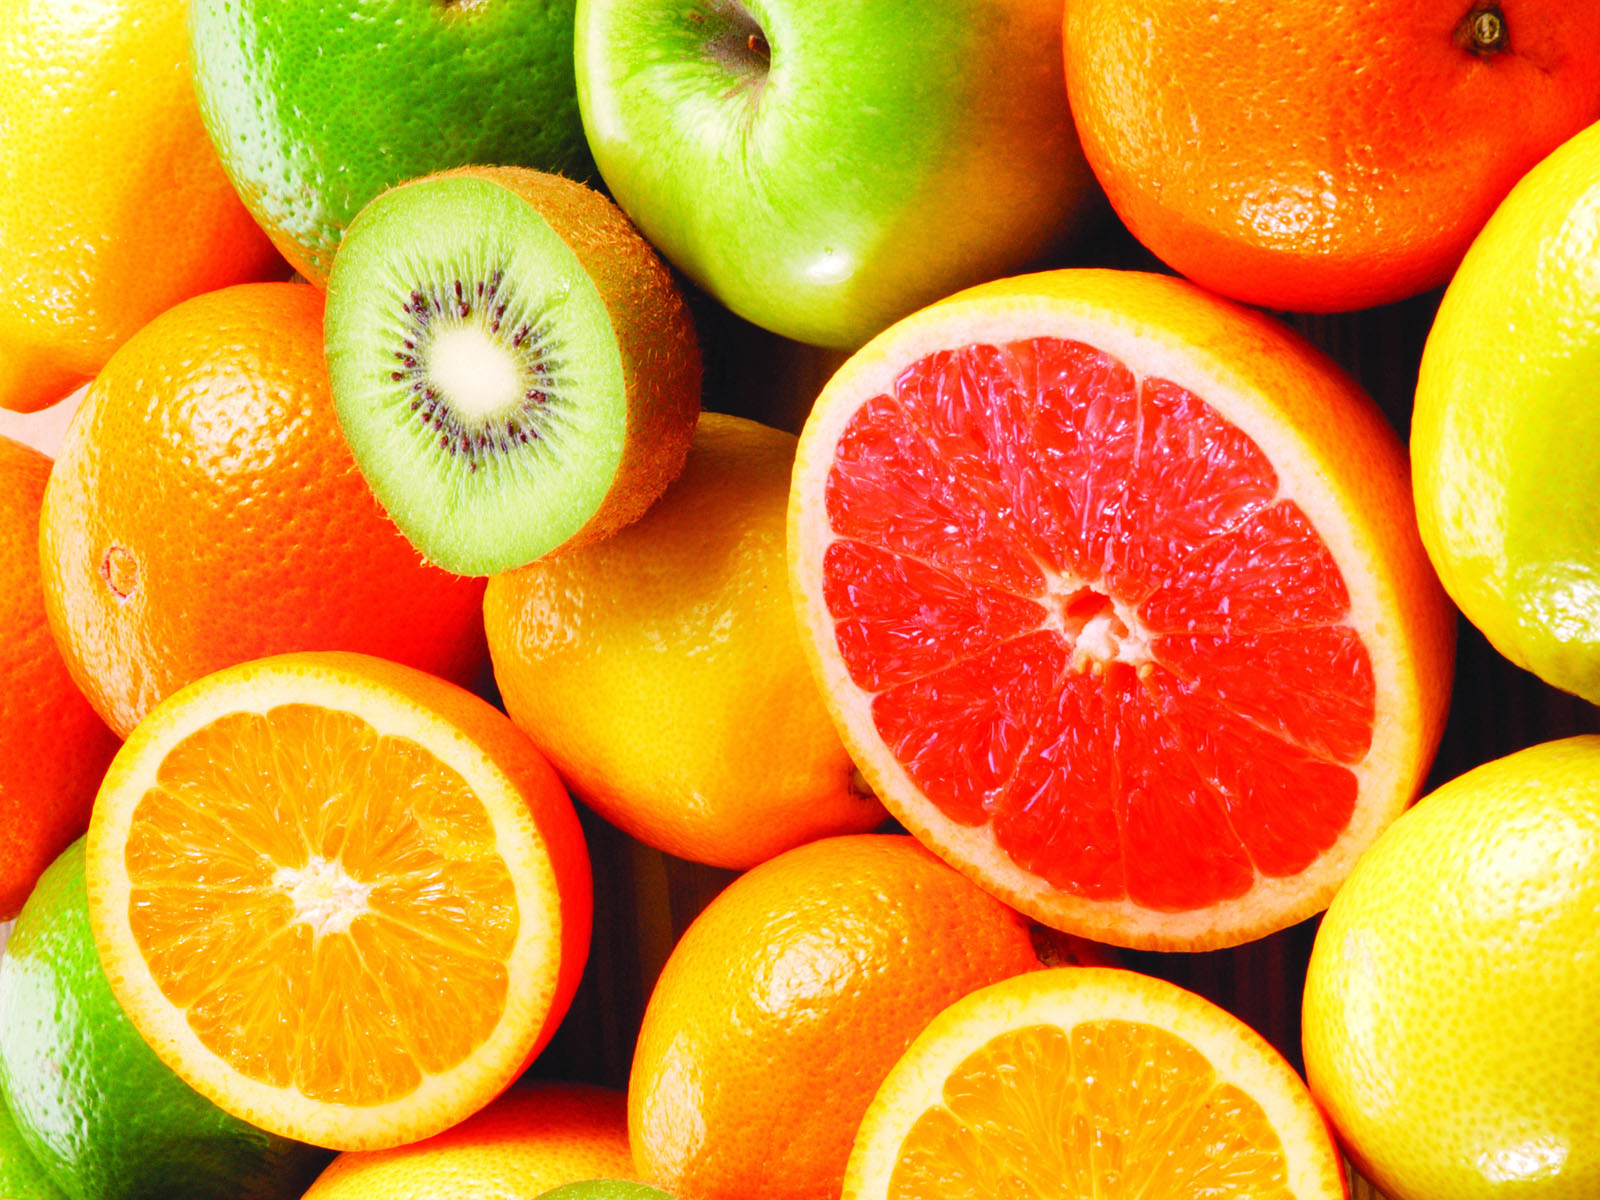
\includegraphics[width=0.3\columnwidth]{fruits}
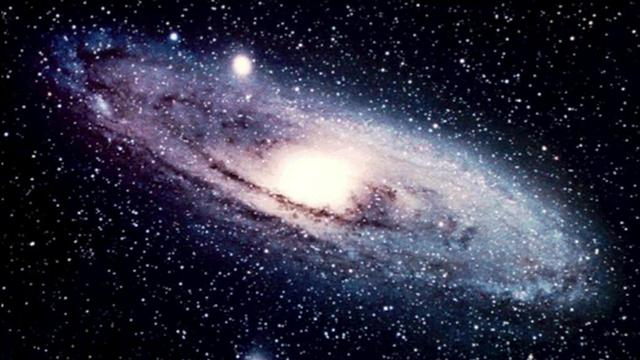
\includegraphics[width=0.3\columnwidth]{galaxy}
%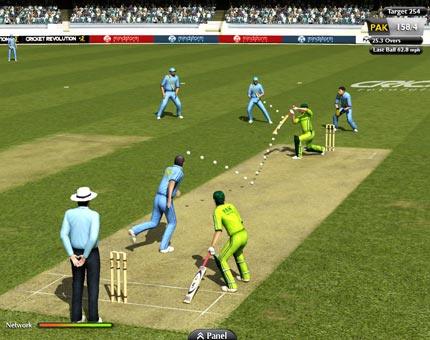
\includegraphics[width=0.3\columnwidth]{webcric}
%\caption{{\color{blue}CT scan image of AAA}}
\end{figure}

%\end{column}
}

%\frame{\frametitle{Example}

\section{Thinking Classes}
\frame{\frametitle{Example}
Make a Computer Game of Cricket.
\begin{columns}[onlytextwidth]
    \begin{column}{0.4\textwidth}
      \centering
\begin{figure}
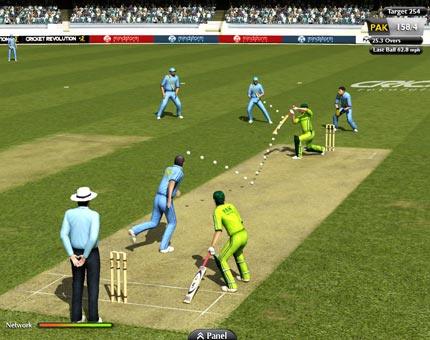
\includegraphics[width=1\columnwidth]{webcric}\\
\end{figure}
    \end{column}
    \begin{column}{0.6\textwidth}
      \centering
      \begin{itemize}
      \item<1-> Teams (Team as Main Class)
      \item<2-> Players (Player as another Class)
      \item<3-> Data defined for each Player tells its characteristics
      \item<4-> Responsibilities and tasks defined as Member functions
      \item<5-> {\color{red}Example Member Functions??}
      \end{itemize}
    \end{column}
\end{columns}
}
\frame{\frametitle{Basic Idea}
  \begin{itemize}
  \item The fundamental idea is to combine into a single unit both {\color{blue}data} and {\color{blue}functions} that operate on the data. 
\item This unit is named as {\color{red}Object}.
\item The definition of this unit is called a {\color{red}Class}.
\item An object’s functions are called {\color{red}member functions} in C++.
\item And its data are called {\color{red}members}
  \end{itemize}
}
\frame{\frametitle{Procedural vs Object Oriented}
  \begin{figure}
    \centering
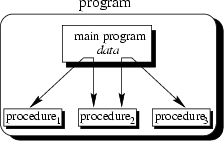
\includegraphics[width=0.4\columnwidth]{procedural.jpg}    
\caption{Procedural Programming}
  \end{figure}
  \begin{figure}
    \centering
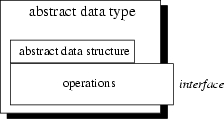
\includegraphics[width=0.4\columnwidth]{abst.jpg}    
\caption{Abstract Data Types-OOP}
  \end{figure}
}
\end{document}


